\documentclass{article}
\usepackage{natbib}
% Language setting
% Replace `english' with e.g. `spanish' to change the document language
\usepackage[english]{babel}

% Set page size and margins
% Replace `letterpaper' with `a4paper' for UK/EU standard size
\usepackage[letterpaper,top=2cm,bottom=2cm,left=3cm,right=3cm,marginparwidth=1.75cm]{geometry}

% Useful packages
\usepackage{amsmath}
\usepackage{graphicx}
\usepackage[colorlinks=true, allcolors=blue]{hyperref}
\usepackage{tikz}
\usetikzlibrary{shapes, arrows, positioning}
\usepackage{longtable}

\title{Literature Review: Systematic Creation of a Cryptocurrency Event Database}

\author{Manoel Gadi}

\begin{document}
\maketitle

\begin{abstract}
Our systematic search was primarily conducted through Google Scholar, a comprehensive academic database that provided the majority of our papers, totaling 39. Google Scholar's extensive collection of scholarly articles ensured that we accessed a wide range of research on cryptocurrency events. To complement this, we utilized the 'IE Library', which contributed two key papers that were selected for their specialized academic content and relevance to our research theme. This was supplemented by a handful of other reputable sources including the International Monetary Fund (IMF), Multidisciplinary Digital Publishing Institute (MDPI), ResearchGate, and Springer, each contributing one paper to our review, thus ensuring a breadth of perspectives and an interdisciplinary approach.

The search within these databases was carefully tailored using specific keywords, publication date ranges, and language filters to ensure that the studies were relevant to our focus on cryptocurrency events. The distribution of the sources reflects a strategic methodology that prioritizes comprehensive coverage while incorporating specialized resources to enhance the depth of the literature review. Each paper was chosen based on a set of inclusion criteria designed to capture the most pertinent and high-quality research in the field.
\end{abstract}

\section{Introduction}

The emergence of cryptocurrencies has introduced a novel dimension to financial markets, blending technological innovation with monetary exchange. This has led to the creation of a vast array of cryptocurrencies, each with its unique features and applications.

\subsubsection{Background}

Cryptocurrencies, from Bitcoin to Ethereum and various stablecoins, have transcended their initial speculative intrigue to become subjects of academic and practical scrutiny. Their unique characteristics, such as decentralization, immutability, and transparency, have made them an interesting subject for research. In particular, the impact of various events on the price and stability of these cryptocurrencies has become a focal point of many studies. However, there is a lack of a comprehensive database that systematically categorizes and records these events. This research aims to fill this gap by creating a systematic cryptocurrency event database, which can serve as a valuable resource for future academic studies and practical applications.

\subsubsection{Research Gap}

Despite extensive discourse, the ability of cryptocurrencies to serve as reliable stores of value during crises remains contested, with studies yielding mixed outcomes on their hedging, diversifying, and safe-haven properties in the face of market volatilities and geopolitical events. This highlights a significant gap in the literature, as the understanding of cryptocurrencies' behavior in crisis situations is crucial for investors, policy makers, and the academic community.

\subsubsection{Objective}

The objective of this review is to systematically create a cryptocurrency event database that can be used to study the performance of cryptocurrencies during different events. By synthesizing existing research, we aim to ascertain whether cryptocurrencies can uphold their value amidst financial crises. This involves drawing from a diverse array of empirical studies that explore their performance against traditional and digital financial indices during periods of economic stress. The creation of such a database will not only contribute to the academic literature but also provide valuable insights for investors and policy makers.

\subsubsection{Methodology Overview}

Employing the PRISMA framework, this review meticulously sifts through 35 selected papers, leveraging both systematic and manual search strategies to encompass a broad spectrum of perspectives on cryptocurrency stability during crises.



\subsubsection{Significance}

The creation of a systematic cryptocurrency event database is of significant importance. It not only provides a comprehensive resource for academic research but also informs investment strategies by offering insights into how different events impact various cryptocurrencies. Furthermore, it guides policy formulation and regulatory frameworks by providing empirical evidence on the behavior of cryptocurrencies in response to different events. This addresses the complexities of integrating digital assets into the global financial ecosystem and aids in the understanding and management of the risks associated with cryptocurrency investments.


\subsubsection{Structure of the Review}

The review is structured to first present the methodology for the systematic creation of the cryptocurrency event database. This includes the data collection process, the criteria for including events in the database, and the classification of events. Following this, we present an analysis of the database, discussing the frequency and types of events, and their impact on different cryptocurrencies. The review culminates in a discussion of the potential applications of the database for academic research, investment strategies, and policy formulation.

This refined introduction provides a comprehensive overview of the scope of your research on the systematic creation of a cryptocurrency event database, informed by the objectives and methodology of your project.


\section{Systematic Search}

The search utilized Boolean operators ("AND"/"OR") with keywords such as "Bitcoin," "Ethereum," "cryptocurrency," "digital currency," "blockchain currency," "cryptoassets," "event study," "event analysis," "event examination," "event investigation," "GDELT," "Google News," "Reuters," "Yahoo," "abnormal return," "positive sentiment," and "negative sentiment." This comprehensive approach aimed to capture a wide range of studies discussing the impact of various events on cryptocurrencies. The specific Google Search prompt used was the following:

("Bitcoin" OR "Ethereum" OR "cryptocurrency" OR "digital currency" OR "blockchain currency" OR "cryptoassets") AND ("event study" OR "event analysis" OR "event examination" OR "event investigation") AND ("GDELT" OR "Google News" OR "Reuters" OR "Yahoo") AND ("abnormal return") AND (("positive" OR  "negative") AND "sentiment")


\subsection{Inclusion Criteria}

The literature review performed by our group was meticulously structured with specific inclusion criteria to ensure the collection of contemporary and pertinent research. We concentrated on scholarly articles published within the last five years, prioritizing the most cutting-edge findings in the rapidly evolving domain of cryptocurrency events. The scope of our review was confined to publications in English, a decision made to facilitate uniform understanding and to cater to the broadest academic audience. This strategy also allowed us to integrate a diverse array of studies while maintaining rigorous standards of research quality and relevance.

Studies were carefully selected based on their direct relevance to cryptocurrency events. This encompassed analyses of market responses to a spectrum of influences including regulatory shifts, geopolitical developments, technological breakthroughs, and influential social media commentary. Methodological soundness was a non-negotiable criterion; only studies exhibiting robust and clearly defined quantitative or qualitative methods were considered, ensuring the dependability of the information presented.

Accessibility was a key factor — our review included only those papers available in full text from the databases searched, which allowed for an in-depth examination of their content and methodologies. Peer-reviewed articles were exclusively considered to guarantee the integrity and scholarly merit of our sources. Lastly, we sought studies presenting a diversity of perspectives — economic, behavioral, technological, and regulatory — to construct a multi-dimensional understanding of the influences shaping the cryptocurrency event landscape. This inclusive yet discerning approach to our literature review criteria guaranteed a collection of studies that were not only relevant and methodologically rigorous but also representative of the varied facets of cryptocurrency events.

\subsection{Exclusion Criteria}

Papers were excluded from our review based on several considerations to ensure the relevance and quality of the included studies:

\begin{itemize}
\item \textbf{Lack of Empirical Data:} Studies that were purely theoretical without providing empirical evidence on the impact of events on cryptocurrency markets were excluded.
\item \textbf{Irrelevance to Cryptocurrency Events:} Papers not directly addressing the influence of external events (e.g., policy changes, geopolitical developments, or social media trends) on cryptocurrency prices, volatility, or trading volumes were omitted.
\item \textbf{Methodological Flaws:} Studies with unclear methodology, insufficient description of data analysis techniques, or those not adhering to standard research practices were excluded. This includes papers without a robust statistical analysis or lacking transparency in the models used.
\item \textbf{Language and Accessibility:} Non-English papers and studies not accessible through standard academic databases or requiring payment for access were excluded to ensure the review's comprehensiveness and reproducibility.
\item \textbf{Duplicate Studies:} In cases where multiple papers from the same authors reported on similar datasets or analyses, only the most comprehensive or recent study was included to avoid redundancy.
\item \textbf{Outdated Information:} Given the fast-paced evolution of the cryptocurrency market, studies published before 2018 were considered outdated unless they provided foundational insights or historical context relevant to contemporary market dynamics.
\end{itemize}


\section{Manual Search}

Besides the systematic search, manual searches were conducted using the IE library search engine and possibly other scholarly databases. This was to ensure that no relevant studies were missed, especially those that might not rank high in Google Scholar but are nonetheless significant to the research topic. Any paper identified through manual search that met the inclusion criteria was added to the literature pool.

\begin{figure}
\centering
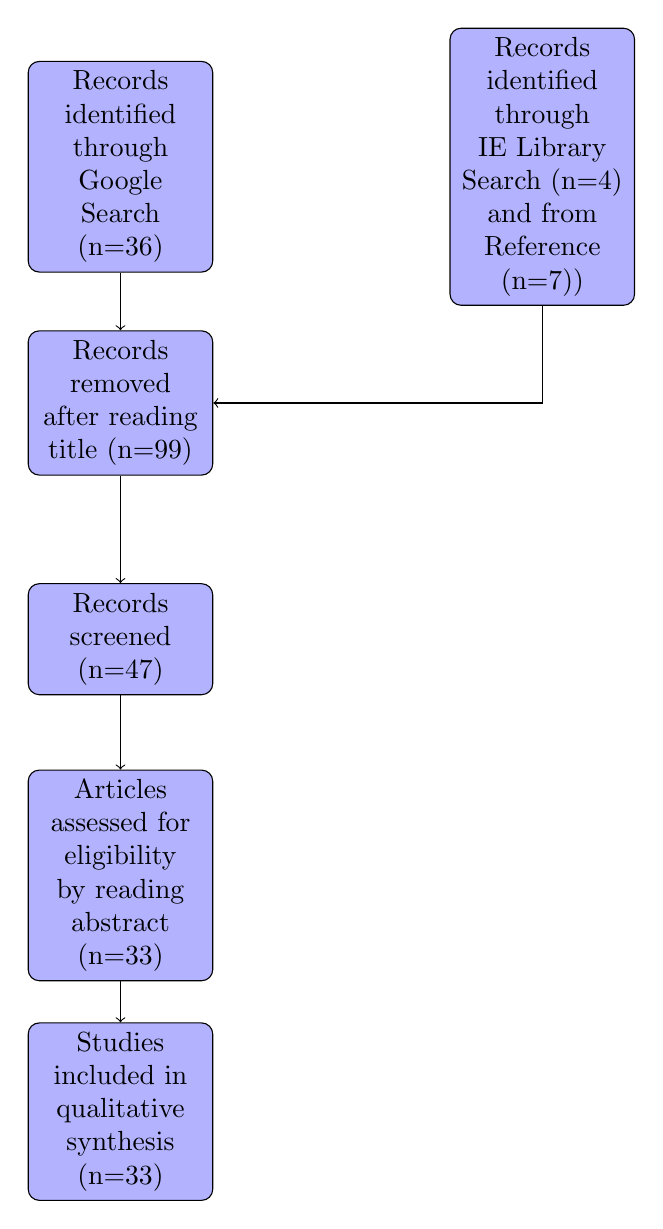
\begin{tikzpicture}[node distance=3cm, auto]
    % Define nodes
    \node (start) [rectangle, rounded corners, text width=6em, minimum height=2em, text centered, draw=black, fill=blue!30] {Records identified through Google Search (n=36)};
    \node (library) [right=of start, rectangle, rounded corners, text width=6em, minimum height=2em, text centered, draw=black, fill=blue!30] {Records identified through IE Library Search (n=4) and from Reference (n=7)) };
    \node (screen1) [below of=start, rectangle, rounded corners, text width=6em, minimum height=2em, text centered, draw=black, fill=blue!30] {Records removed after reading title (n=99)};
    \node (screen2) [below of=screen1, rectangle, rounded corners, text width=6em, minimum height=2em, text centered, draw=black, fill=blue!30] {Records screened (n=47)};
    \node (eligible) [below of=screen2, rectangle, rounded corners, text width=6em, minimum height=2em, text centered, draw=black, fill=blue!30] {Articles assessed for eligibility by reading abstract (n=33)};
    \node (included) [below of=eligible, rectangle, rounded corners, text width=6em, minimum height=2em, text centered, draw=black, fill=blue!30] {Studies included in qualitative synthesis (n=33)};

    % Connect nodes
    \draw[->] (start) -- (screen1);
    \draw[->] (library) |- (screen1);
    \draw[->] (screen1) -- (screen2);
    \draw[->] (screen2) -- (eligible);
    \draw[->] (eligible) -- (included);
\end{tikzpicture}
\caption{PRISMA Flow Diagram of the Literature Review Process}
\end{figure}

\section{Table of Reviewed Studies}
\begin{longtable}{|p{2.0cm}|p{2cm}|p{2.5cm}|p{3.8cm}|p{5.0cm}|}
\caption{Summary of Reviewed Studies} \label{table:studies} \\
\hline
\textbf{Ref.} & \textbf{Title} & \textbf{Data / Sample} & \textbf{Methodology} & \textbf{Results} \\
\hline
\endfirsthead

\multicolumn{5}{c}%
{{\bfseries Table \thetable\ continued from previous page}} \\
\hline
\textbf{Ref.} & \textbf{Title} & \textbf{Data / Sample} & \textbf{Methodology} & \textbf{Results} \\
\hline
\endhead
\hline \multicolumn{5}{|r|}{{Continued on next page}} \\ \hline
\endfoot
\hline
\endlastfoot
\cite{sawhney2021quantitative} & Quantitative Day Trading From Natural Language using Reinforcement Learning & English tweets and Chinese financial news related to major stock indexes and markets. & The study introduces PROFIT, a deep reinforcement learning (RL) approach leveraging financial news and tweets for stock trading. It involves modeling market information hierarchically to learn temporally relevant signals from textual data and optimize trading actions towards profit generation. & PROFIT model outperforms state-of-the-art models in terms of risk-adjusted returns by over 13\% and minimizes extreme losses by over 16\%. The approach demonstrates practical and real-world applicability, showcasing the effectiveness of using natural language processing and reinforcement learning in quantitative day trading strategies. \\
\hline
\cite{chevapatrakul2018detecting} & Detecting overreaction in the Bitcoin market: A quantile autoregression approach & Bitcoin price data from April 29, 2013, to July 3, 2018, covering 1892 daily, 270 weekly, and 62 monthly return observations. & Utilizes quantile autoregression (QAR) models to explore the persistence of Bitcoin returns across different parts of the return distribution and detect overreaction in the market. & Evidence of overreaction was found, with investors tending to overreact during days of sharp price declines and weeks of market rallies, suggesting inefficiencies in the Bitcoin market. \\
\hline
\cite{pyo2019fomc} & Do FOMC and macroeconomic announcements affect Bitcoin prices? & Bitcoin prices and announcement dates of FOMC and macroeconomic variables from July 18, 2010, to September 10, 2018. & The study uses regression models to analyze the effect of FOMC and macroeconomic announcements (employment rate, CPI, PPI) on Bitcoin prices, incorporating GARCH(1,1) for volatility modeling. & The research finds that Bitcoin prices are significantly affected by FOMC announcements, particularly showing an increase the day before and a decrease on the announcement day, but finds no significant effects from macroeconomic announcements. \\
\hline
\cite{sawhney2022cryptocurrency} & Cryptocurrency Bubble Detection: A New Stock Market Dataset, Financial Task \& Hyperbolic Models & Dataset comprises over 400 cryptocurrencies from 9 exchanges over five years, with over two million tweets. & Multi-span identification using sequence-to-sequence hyperbolic models, with a dataset curated from social media and financial sources. The methodology includes data mining, bubble creation analysis, and zero-shot learning. & The models demonstrated improved performance in detecting speculative bubbles by leveraging social media data, and showed generalizability to new, unseen data from Reddit under zero-shot conditions. \\
\hline
\cite{shanaev2022cryptocurrency} & Cryptocurrency value and 51\% attacks: evidence from event studies & 14 individual attacks across 13 cryptocurrencies. & The study employs event study methodologies to analyze the price impact of 51\% attacks on cryptocurrencies, using an exhaustive sample of attacks and applying multiple statistical techniques to ensure robustness. & Consistent negative price response to 51\% attacks, with coin prices falling 12-15\% immediately after the attack and not recovering within a week, indicating the market's efficiency in processing such events. \\
\hline
\cite{gadi2022cryptocurrency} & Cryptocurrency Curated News Event Database From GDELT & Over 243,000 cryptocurrency-related news events from GDELT between March 2021 and April 2022. & The dataset was enhanced with supervised machine learning models to assign relevance, sentiment, and strength scores to news events. The authors compare several models and utilize Naive Bayes and FinBERT for final scoring. & The results indicate that using a curated database like GDELT for news events provides a more balanced perspective compared to selecting news from cryptocurrency-specific websites. The dataset and associated Jupyter Notebooks are made available for public use. \\
\hline
\cite{kremser2019large} & How Do Large Stakes Influence Bitcoin Performance? Evidence From The Mt.Gox Liquidation Case & The study analyzes 787,308 tweets from January 2016 to April 2018. & Sentiment analysis of Twitter data and vector error correction model analysis to understand the long-run relationships between variables. & The study confirms a positive association of Bitcoin performance with positive Twitter sentiment and tweet volume, and a negative association with negative sentiment. It also provides empirical evidence of a lasting negative impact of Mt.Gox selloff events on Bitcoin price, which can be measured using Twitter sentiment and tweet volume. \\
\hline
\cite{park2020global} & Global Bitcoin Markets and Local Regulations & Six major Bitcoin trading markets & Event study methodology, analyzing the impact of regulatory events on Bitcoin prices and trading volumes by examining changes around the announcement dates of regulation events. & Regulatory events have a transient effect on Bitcoin prices and a more prolonged dampening effect on trading volumes. The openness of financial markets can lessen the negative impact of domestic regulations. \\
\hline
\cite{gnazzo2022political} & Political Risk and the Cryptocurrency Market: An Application on the Russian Invasion of Ukraine & 99 tokens listed on CoinGecko & The study employs an event study methodology, leveraging the Russian invasion of Ukraine as an exogenous shock to the cryptocurrency market. It calculates the cumulative abnormal returns (CAR) over several time windows (one day, four days, one week, two weeks, three weeks, and a month) to analyze the market's reaction to the invasion. & The study found cryptocurrencies underperformed in the immediate aftermath of the invasion but showed greater returns over extended periods, particularly for cryptocurrencies with longer market tenures. \\
\hline
\cite{mnif2021covid} & COVID-19, Bitcoin Market Efficiency, Herd Behaviour & Bitcoin cryptocurrency between April 19, 2013, and May 5, 2020 & Multifractal Detrended Fluctuation Analysis (MFDFA) and an event study methodology to assess market efficiency and herd behavior in response to COVID-19. Utilizes statistical measures such as the Generalized Hurst exponent and the inefficiency index (MLM). & Bitcoin showed multifractality and was more efficient post-pandemic, indicating reduced herd bias. \\
\hline
\cite{strukov2021elon} & How Elon Musk’s Statements in Social Media Move Cryptocurrency Market & Bitcoin and Dogecoin cryptocurrencies, focusing on specific tweets by Elon Musk & Event study methodology analyzing the impact of Elon Musk's tweets on the price and trading volumes of Bitcoin and Dogecoin. Utilizes statistical analysis to measure the immediate and subsequent effects on the cryptocurrency market. & Musk's tweets had a significant impact on both Bitcoin and Dogecoin, causing immediate price fluctuations and increased trading volumes, demonstrating the influence of social media on cryptocurrency markets. \\
\hline

\cite{praveena2020coronavirus} & Coronavirus Spreads and Bitcoin’s 2020 Rally: Is There a Link? & Bitcoin market data from January 01, 2018, to February 15, 2020 & Utilizes a dynamic event-study methodology with a Generalized Autoregressive Conditionally Heteroskedastic (GARCH) model to examine Bitcoin's response to the onset of coronavirus, analyzing cumulative abnormal returns and volatility. & Finds that coronavirus has exacerbated Bitcoin's volatility and had a complex impact on its prices, with an initial underreaction followed by a significant reaction over time, challenging the efficient market hypothesis. \\
\hline
\cite{aggarwal2019understanding} & Understanding the Social Factors Affecting the Cryptocurrency Market & The sample in the study involves recording dates of significant peaks and drops in cryptocurrency prices over six months (Nov 1st 2017 to April 30, 2017). Data were collected on the top news stories a day before each major peak or drop, under the assumption that this news influenced the subsequent price movement. & The methodology includes sentiment analysis, correlation analysis to identify significant factors affecting market prices, and validation of these factors through real-time social media data analysis. & Social factors have varying correlations with cryptocurrency prices: tech personalities' opinions and regulatory news often negatively influence prices, while government regulation has a complex, sometimes positive effect. The research identifies gaps in data across geographies and languages and the difficulty in measuring the precise effects of news on market prices, given the complex factors at play. \\
\hline
\cite{huynh2022essays} & Essays on market reaction and cryptocurrency & The sample comprises daily Bitcoin price data from CoinMarketCap (May 1, 2013, to October 28, 2019) and Gold and Platinum prices from Thomson Reuters, with analyses based on natural logarithm daily returns and constructed average monthly Bitcoin returns to study its role as an alternative investment. (Chapter 4 only) & Wavelet multiple correlation and quantile regression (Chapter 4) & The GP ratio is a significant predictor of Bitcoin returns, with positive coefficients across different models indicating that an increase in the GP ratio is associated with an increase in Bitcoin returns. The analysis found that the predictive power of the GP ratio on Bitcoin returns is robust across 1, 3, 4, and 12 months. Gaps: The research suggests further investigation into the dynamic relationship between precious metals and cryptocurrencies, particularly under different economic conditions and policy change \\
\hline
\cite{caferra2020good} & Good vibes only: The crypto-optimistic behavior & The sample consists of 730 daily observations from January 1, 2018, to January 1, 2020, across 13 cryptocurrencies (including Bitcoin, Ethereum, and Ripple) sourced from Yahoo Finance, and media coverage data on these cryptocurrencies from the GDELT Project, focusing on periods excluding extreme market events like the 2017 bubble burst and COVID-19. & Sentiment analysis, employing both Cross-sectional standard (CSSD) and absolute (CSAD) deviation & Findings indicate that more optimistic news correlates with lower returns dispersion, suggesting a convergence of investor beliefs. This highlights the significant role of media sentiment in influencing cryptocurrency market dynamics. However, the study points to limitations in establishing causal relationships between news sentiment and market prices, suggesting future research could further explore these dynamics. \\
\hline
\cite{frydendahl2019media} & How media coverage news and global uncertainties drive forecast of cryptocurrencies returns? & Daily price data for Bitcoin and Ethereum from January 30, 2020, to April 26, 2021 & Event study methodology; It employs the Quantile-on-Quantile (QQA) approach & Significant negative effects of Economic Policy Uncertainty and COVID-19 news coverage on cryptocurrency returns \\
\hline
\cite{chokor2020long} & Long and short-term impacts of regulation in the cryptocurrency market & The impact of regulatory events on the returns of the top thirty cryptocurrencies by market capitalization from 2015 to 2019 & Event study to assess the impact of regulatory events on cryptocurrency returns, complemented by cross-sectional analysis & Regulatory events are generally followed by negative abnormal returns \\
\hline
\cite{jarboui2021cryptocurrency} & Cryptocurrency bubble risk and the FOMC announcements during COVID-19 black swan event & The top five cryptocurrencies by market capitalization (Bitcoin, Ethereum, Tether, Litecoin, and Ripple) from 01 January 2020 to 5 November 2020 & Event study methodology to analyze the effects of Federal Open Market Committee (FOMC) announcements on cryptocurrency dynamics and investigates the presence of bubbles using the PSY test & Significant negative effect on the studied cryptocurrencies (except Tether) following the first FOMC announcement \\
\hline

\cite{panagiotidis2018effects} & The effects of markets, uncertainty and search intensity on bitcoin returns & Bitcoin returns using daily data, assessing the impact of stock market returns, exchange rates, gold and oil returns, Federal Reserve and European Central Bank rates, and internet search trends & Utilizes VAR (Vector Autoregressive) and FAVAR (Factor-Augmented Vector Autoregressive) models & Significant interactions between Bitcoin and traditional stock markets, a weaker relationship with foreign exchange markets and the macroeconomy, and a diminished importance of internet search trends on Bitcoin returns \\
\hline
\cite{garcia2021bibliometric} & A Bibliometric Review of Cryptocurrencies & Articles from Web of Science and Scopus, 2010-early 2019 & Bibliometric analysis using Tableau R, Bibliometrix R Package, and VOSviewer & Maps the growth and trends in cryptocurrency research, identifying key areas and global contributions \\
\hline
\cite{kerner2021crypto} & Crypto-asset Database and Indicators at the ECB & Crypto-assets data monitored by the ECB & Development of a monitoring framework and indicators & Enhances the understanding of crypto-assets' impact on financial stability and policy \\
\hline
\cite{theiri2022cryptocurrency} & Cryptocurrency liquidity during the Russia–Ukraine war: the case of Bitcoin and Ethereum & Liquidity of Bitcoin and Ethereum during the Russia-Ukraine war, using high-frequency hourly transaction data from 1 February 2022 to 31 March 2022 & An event study methodology was applied, evaluating hourly transactions of Bitcoin and Ethereum over the designated period & A significant but temporary impact of the Russia–Ukraine war on the liquidity of Bitcoin and Ethereum \\
\hline

\cite{przyluska2023dynamics} & The Dynamics of Cryptocurrency Price Volatility in the Face of the Crisis on the Example of Bitcoin and Ethereum & Bitcoin and Ethereum price fluctuations from January 2021 to June 2022 & Empirical data analysis, time series analysis, Pearson’s correlation, chi-square test, and descriptive statistics & Significant and unpredictable fluctuations in cryptocurrency prices, especially during market shocks \\
\hline
\cite{kostika2020dynamic} & Dynamic linkages among cryptocurrencies, exchange rates and global equity markets & Bitcoin, Dash, Ethereum, Monero, Stellar, and XRP, alongside major exchange rates and global stock market indices from 2013 to 2018 & Vector Autoregressive (VAR) model and Engle’s Dynamic Conditional Correlation Generalized Autoregressive Conditional Heteroskedasticity (DCC-GARCH) specification & Weak correlations among cryptocurrencies and between cryptocurrencies and other financial assets \\
\hline
\cite{park2020diffusion} & Diffusion of cryptocurrencies: web traffic and social network attributes as indicators of cryptocurrency performance & Top 50 cryptocurrency websites based on market capitalization & Webometrics and social network analysis, including citation analysis and big data analytics & Significant correlations between web traffic, social network attributes, and cryptocurrency market indicators \\
\hline
\cite{tomic2020measuring} & Measuring the effects of Bitcoin forks on selected cryptocurrencies using event study methodology & Eight major cryptocurrencies, selected based on market capitalization and existence during the estimation windows, excluding stable-coins & Event study methodology, incorporating regression analysis and various statistical tests & No statistically significant negative abnormal returns for Bitcoin Cash's creation. However, statistically significant negative effects on the market due to the forks that led to the creation of Bitcoin Gold and Bitcoin SV \\

\cite{katsiampa2019} & An empirical investigation of volatility dynamics in the cryptocurrency market & Daily closing prices of Bitcoin, Ether, Ripple, Litecoin, and Stellar Lumen from August 2015 to February 2018. & Asymmetric Diagonal BEKK model to study volatility dynamics, including the assessment of asymmetric effects and time-varying conditional correlations. & The study found that cryptocurrencies' volatility dynamics are significantly affected by past shocks and that their conditional covariances reflect asymmetric effects of these shocks. Time-varying conditional correlations were also observed, with cryptocurrencies' volatility dynamics found to be responsive to major news events. \\
\hline
\cite{rognone2020} & News Sentiment in the Cryptocurrency Market: An Empirical Comparison with Forex & High-frequency intra-day data from January 2012 to November 2018, including Bitcoin and major traditional currencies. & The study uses a Vector Autoregression with Exogenous Variables (VAR-X) model to examine the effects of news sentiment on currency returns, volume, and volatility. & Bitcoin exhibits a distinctive reaction to news compared to traditional currencies, reacting positively to both positive and negative news and displaying investor enthusiasm, particularly during bubble periods. \\
\hline
\cite{ali2023} & Effect of blockchain technology initiatives on firms’ market value & Blockchain project announcements by U.S. firms, totaling 114 firm-event observations. & Event study methodology to analyze short- and long-term market reactions to blockchain initiative announcements. & Positive short-term market reactions to blockchain announcements, especially for projects aimed at saving costs or time, and from smaller firms. Long-term effects on operating performance were found to be non-significant. \\
\hline
\cite{schleiss2018} & How Markets Value The Blockchain Technology: An Empirical Analysis & Publicly traded companies announcing blockchain-related name changes between December 2015 and June 2018. & Event study to analyze cumulative abnormal returns around the announcement days of blockchain name changes. & Significant positive stock market reactions to blockchain name changes, demonstrating the market's valuation of blockchain technology without significant long-term impact on operating performance. \\
\hline

\cite{hassani2018bigcrypto} & Big-Crypto: Big Data, Blockchain and Cryptocurrency & Not specific; the paper reviews broader trends and developments in cryptocurrency and Big Data research & Systematic review of literature and technological developments in Big Data and cryptocurrency post-2016 & The paper identifies and summarizes interactions between Big Data and cryptocurrency, focusing on security, privacy enhancement, analyses, and prediction \\
\hline
\cite{kamal2023cryptocurrencies} & Cryptocurrencies and the Threat vs. the Act Event of Geopolitical Risk & Top 5 and Top 100 cryptocurrencies based on market capitalization & The study uses an event study methodology analyzing hourly data from Binance & Both threat and act events decreased liquidity and returns, with act events showing a more significant impact \\
\hline
\cite{naifar2023president} & President Trump, his tweets, and the stock market & President Donald J. Trump's tweets targeting specific companies from November 8, 2016, to February 20, 2019, alongside daily closing stock prices for 30 companies listed on 8 different stock exchanges & Sentiment analysis, employing both Cross-sectional standard (CSSD) and absolute (CSAD) deviation of returns & Positive tweets generally lead to immediate positive stock price reactions, while negative tweets result in delayed negative impacts \\
\hline

 \end{longtable}

\section{Results, Discussion and Gap Found}

In our examination, it becomes evident that the relationship between worldwide phenomena and economic policies plays a crucial role in defining the contours of the cryptocurrency market. This analysis highlights how these factors intertwine to influence market behavior, volatility, and investor sentiment, offering insights into the underlying mechanisms driving cryptocurrency dynamics. Investigations into macroeconomic pronouncements, such as those emanating from the FOMC, have divulged their substantial, although frequently adverse, sway over the cryptocurrency exchanges, especially in the throes of global upheavals akin to the COVID-19 contagion, as dissected by \cite{jarboui2021}.  Despite revelations, the extant literature tends to hone in on the immediate repercussions to market stimuli, leaving a lacuna in the understanding of their sustained effects. This gap underscores a scholarly avenue ripe for exploration, aiming to illuminate the long-lasting influences of such events, thereby enriching the comprehensive narrative of cryptocurrency market dynamics.

The synthesis of findings from our literature review also indicates a robust interest in the relationship between public sentiment, media coverage, and market movements in the cryptocurrency space. The responsiveness of cryptocurrencies to influential figures' statements on social media, as demonstrated by the significant market fluctuations following Elon Musk's tweets, underscore the intersection of technology, market psychology, and investment strategies in the digital age. However, while such events provide immediate insights into market sentiment and reaction, there remains an underexplored area regarding the aggregate effect of these disparate events on the long-term stability and adoption of cryptocurrencies.

Moreover, the studies reviewed often highlight the potential of cryptocurrencies as alternative investments or hedges against traditional financial systems and assets. However, this purported role is consistently challenged by empirical findings that suggest a more complex reality. For instance, the investigation into Bitcoin's performance during the Russian invasion of Ukraine by \cite{gnazzo2022} illustrates the resilience of the cryptocurrency market to geopolitical shocks, albeit with nuanced performance across different tokens and timeframes.

Collectively, the reviewed literature offers valuable perspectives on the immediate effects of socioeconomic and geopolitical events on cryptocurrency markets. However, it also reveals a significant gap in our understanding of the long-term implications of these events. As the body of research grows, there is a critical need for comprehensive studies that consider a wider array of variables, including the cumulative impact of regulatory changes, technological advancements, and evolving market sentiments, to provide a more holistic view of the cryptocurrency ecosystem and its future trajectory.


\bibliographystyle{plainnat}
\bibliography{sample}

\end{document}